% MSc dissertation example file, February 2022
%
% Leave one of the documentclass lines uncommented to match your degree.
% You may remove the logo option if it causes problems.
% Do not change any other options.
% \documentclass[logo,msc,adi]{infthesis}     % Adv Design Inf
% \documentclass[logo,msc,ai]{infthesis}      % AI
% \documentclass[logo,msc,cogsci]{infthesis}  % Cognitive Sci
% \documentclass[logo,msc,cs]{infthesis}      % Computer Sci
% \documentclass[logo,msc,cyber]{infthesis}   % Cyber Sec
% \documentclass[logo,msc,datasci]{infthesis} % Data Sci
% \documentclass[logo,msc,di]{infthesis}      % Design Inf
% \documentclass[logo,msc,dsti]{infthesis}    % Data Sci TI
% \documentclass[logo,msc,inf]{infthesis}     % Informatics
\documentclass[logo,msc]{infthesis}           % degree unspecified, do not change except to add your degree
%%%%%%%%%%%%%%%%%%%%%%%%
% Understand any problems and seek approval before assuming it's ok to remove ugcheck.
\usepackage{msccheck}

% Include any packages you need below, but don't include any that change the page
% layout or style of the dissertation. By including the ugcheck package above,
% you should catch most accidental changes of page layout though.
\documentclass{article}
\usepackage{mathtools}
\usepackage{microtype} % recommended, but you can remove if it causes problems
\usepackage{graphicx}
\usepackage{subfig}

\begin{document}
\begin{preliminary}

\title{Machine Learning of Polyhedral Compilation}

\author{Prakshal Nandi}

\date{\today}

\abstract{
In most compute-intensive applications, a significant amount of time is spent on the execution of the loops. Compilers like clang offer many optimisation options such as loop tiling, unrolling, vectorization or parallel processing. Most optimizations are still particular to the loop they are trying to transform and require specific knowledge in this domain. If the loops follow a specific structure, it is possible to change the execution order of the loop statements to make the program run faster. But finding a profitable schedule at the compile time is a complex task, as there are lots of constraints and dependencies involved.

Fortunately, using the OpenAI Gym interface, PolyGym \cite{P1} has converted this problem into an environment of optimizations for Reinforcement Learning algorithms. The loops are converted into polyhedral representation, upon which different transformations can be applied. This thesis explores the feasibility of using a Reinforcement Learning agent to find a profitable schedule. First, we generate valid schedules using agent-chosen actions transforming the polyhedral model. Secondly, we are doing a search in the space of the possible schedule to find the optimal solution using a different RL agent. Finally, with the help of some experiments, we show how different RL algorithms perform, starting from basic Q-Learning algorithm to more advanced and popular deep reinforcement learning algorithms.
}

\maketitle

\newenvironment{ethics}
   {\begin{frontenv}{Research Ethics Approval}{\LARGE}}
   {\end{frontenv}\newpage}

\begin{ethics}
This research does not involve any human participants or personal data. All data are collected based on simulation experiments on benchmark suites; hence no ethical concerns are associated with the project.

\standarddeclaration
\end{ethics}


\begin{acknowledgements}
Any acknowledgements go here.
\end{acknowledgements}


\tableofcontents
\end{preliminary}


\chapter{Introduction}

\section{Motivation}

Reinforcement Learning(RL) has recently been seen as a promising approach for compiler optimization \cite{8357388}\cite{9232934}. A Reinforcement Learning agent makes the \textit{observations} within the \textit{environment}, and takes \textit{actions} to receive certain \textit{rewards}. The goal is to maximize the rewards over a period of time. On the other side, the space of the possible transformations available to a compiler is vast to achieve optimizations related to data locality, memory management, communication, and automatic parallelization. Applying Machine Learning(ML) algorithms to find a good strategy in this space is challenging. Polyhedral Compilation is one type of compiler optimization technique applicable to a particular class of nested loops. It can explore geometric dependency properties of kernel statements in different iterations and apply transformations to improve the schedule of the loop execution. In compiler optimization, machine learning is yet to achieve the level of success in other fields such as Computer Vision or Natural Language Processing. Even though it has been an object of research for more than two decades, machine learning guided techniques are still not widely utilized in industrial compilers.



\section{Objectives}

The aim of the project is to analyze how Reinforcement Learning can help improve Polyhedral Compilation. This analysis will be performed with the help of Deep Neural Networks and other hybrid meta-heuristics. The research hypothesis is that Reinforcement Learning algorithms can be generalized to learn Polyhedral Compilation.

It is not always clear how to represent the actual problem in a Reinforcement Learning environment. However, this part has already been covered in Polygym\cite{9563041}; hence it is not going to be the focus of this research. The main objectives for this project are trying to find answers to these questions:
\begin{itemize}

    \item Can we implement a Deep Reinforcement Learning algorithm that can help select the best actions related to polyhedral transformations? 
    \item Can we design reward functions that improve the training performance to learn profitable schedules?
    \item Can we explore different RL algorithms and find the most suitable technique by evaluating their performance?


\end{itemize}

\section{Structure}

This project proposal is structured as follows: Following the discussion regarding the problem statement, research objective, novelty, and significance of the project in Section 1, Section 2 provides an overview of the background and literature review. Section 3 focuses on project methodology, limitations, risks, and ethical considerations. Section 4 explains how the evaluation of the developed methods will be carried out. Section 5 discusses expected outcomes, and Section 6 outlines the research timeline, milestones, and deliverables.

\chapter{Background}

\section{Polyhedral Compilation Model}

In Figure \ref{fig:Polly_Loop}, a simple two-dimensional loop nest is shown. There are different ways in which this loop can be optimized, including changing the order execution, cache locality, data location, vector instructions, parallel threads and tasks. The execution of this loop next can be executed in the order shown in \ref{fig:Loop_Schedule}. The individual operation which we execute can be written down as a point in a two-dimensional vector space, Figure \ref{fig:Loop_Str}. In general, there are more than two dimensions. We could generalise this representation as a polyhedron to more concisely represent this set of points. This polyhedron can be described as a set of linear constraints we must adhere to while applying the transformations, \ref{fig:Loop_Ineq}. Thus, an n-dimensional mathematical model like polytope can be used to represent the iteration space of a nested loop \cite{P3}. The iteration space of the loop nest can be described as in the Equation \ref{eq:I_space}. The time when these iterations are performed, i.e. the schedule, can be described as in Equation \ref{eq:S_space}.  If we want to change the behaviour of how the program runs, we only need to change this execution schedule. Notably, the loop interchange can be implemented here by just changing the schedule from \textit{(i,j)} to \textit{(j,i)}.

\begin{equation}
I_s = \{S(i,j) \hspace{2} | \hspace{2} 1 <= i <= n \hspace{2} and \hspace{2} 1 <= j <= i\}
\label{eq:I_space}
\end{equation}

\begin{equation}
\theta_s = \{S(i,j) \hspace{2} \Rightarrow (i,j) \}
\label{eq:S_space}
\end{equation}

The optimization through Polyhedral Compilation is achieved in three different stages, moving from code to polyhedron model, applying program transformations within the model, and finally regenerating the code from the model. This model gives the framework to transform the loops, where the array references and loop bounds are affine functions of loop iterators and parameters. The polyhedral model is broadly applicable due to the high presence of affine loops in compute-bound applications\cite{poly_applicable}. In the kernel example shown in Figure 1, geometric interpretations such as two-dimensional polygons can be used to visualize dependencies between statements. Based on these dependencies, conclusions can be made regarding the preferred execution time of each statement. 

\begin{figure}[!tb]
  \centering
  \subfloat[Polly Loop.]{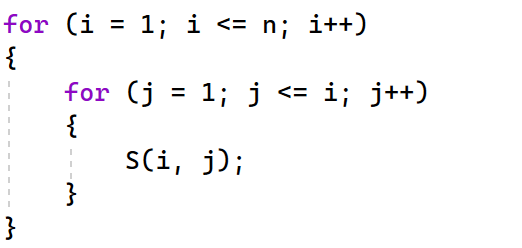
\includegraphics[width=0.5\textwidth]{Images/polly_loop.png}\label{fig:Polly_Loop}}
  \hfill
  \subfloat[Structure of loop.]{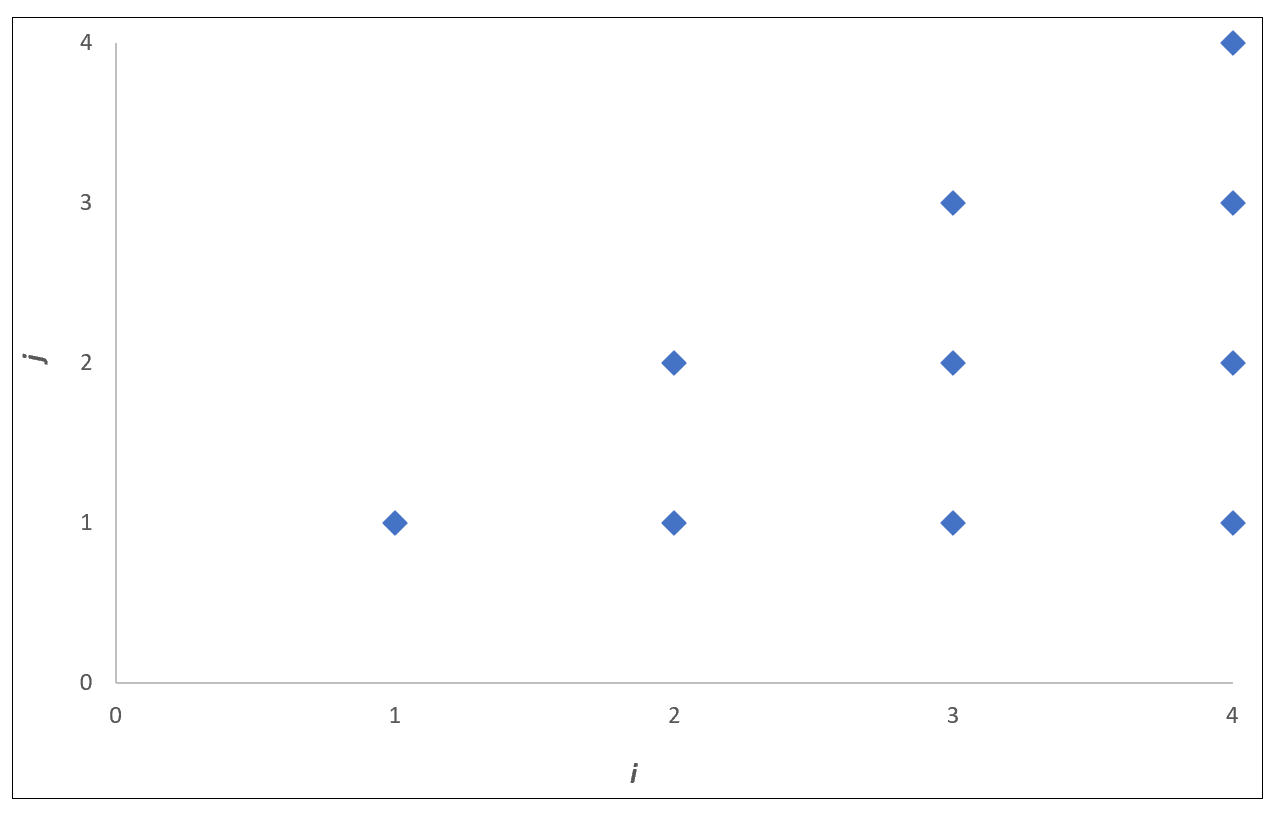
\includegraphics[width=0.5\textwidth]{Images/loop_structure.png}\label{fig:Loop_Str}}

  \centering
  \subfloat[Schedule of Loop Execution]{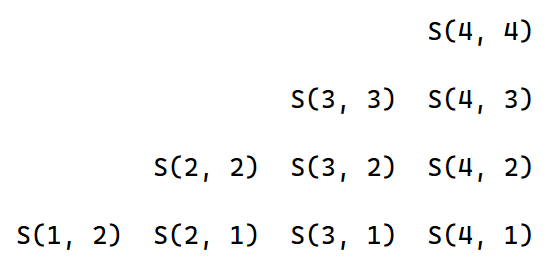
\includegraphics[width=0.5\textwidth]{Images/loop_schedule.png}\label{fig:Loop_Schedule}}
  \hfill
  \subfloat[Loop Inequalities]{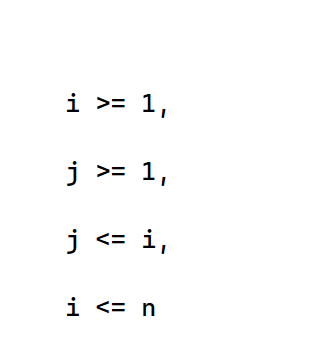
\includegraphics[width=0.45\textwidth]{Images/loop_inequalities.png}\label{fig:Loop_Ineq}}
  
  \caption{Polyhedral Representation of Loop Execution}
\end{figure}

\section{Deep Reinforcement Learning}

The problem of reinforcement learning can become challenging if the number of states possible in the environment is too vast. Deep Learning addresses this challenge by approximating the Q-values of the state and action pairs, using model parameters called weights. The framework of deep learning is made of the neural network, consisting of an input layer, an output layer and one or more intermediate layers. The neurons in the layer have weights associated with 
them, which we are trying to optimize. The output generated by the network is compared with the target, and loss will be calculated. Different loss functions are available for comparisons, such as mean square error, cross-entropy loss or maximum likelihood loss. They all represent how far is the output of the model with respect to the desired result. Once we know the loss value, the gradients can be calculated considering the effect of each parameter on the output. Using an optimizer, such as SGD, Adam, or RMSprop, we can change the weight values to reduce the loss using the calculated gradients. We are moving towards the desired result by doing this in an iterative manner. Performing all these steps manually could be useful in understanding how deep learning works, but it could be extremely difficult in practical application. Luckily, we have libraries such as PyTorch available, which can calculate the gradients and perform backpropagation (may be more) to develop new network parameters.

\section{PyTorch}

PyTorch implements a dynamic graph approach for gradient calculation, where the library keeps track of the operations performed on the data, and unrolls this operation sequence when we need to calculate the associated gradients. The basic building block of DL is the \textit{tensor}, representing a multi-dimensional array, which is also implemented by this toolkit. PyTorch has methods to create tensors, convert numpy arrays to tensors, and generate tensors with specific data, such as \textit{torch.ones()}. It can also apply different operations on the tensors to concatenate, resize and transpose them. The library also allows for offloading the tensor calculations to GPU by specific the \textit{}device property associated with it. A tensor may or may not have gradient construction available to it, which can be configured and retrieved using properties such as \textit{requires\_grad} and \textit{grad}. By using \textit{backward} operation, we can ask PyTorch to calculate the gradients of all the variables in the network. By leveraging \textit{nn.Module} of PyTorch, we can define the network architecture, design dropouts, reinitiate the gradients and apply transformations such as \textit{Softmax} (may be more).

\section{PolyGym}

The geometric properties of the dependencies between two statements during loop iteration execution can be defined in the form of space of constraints. Exploration of this space offers an opportunity to apply semantics-preserving transformations to improve the performance of the loop. This exploration mainly has two methods: problem-specific heuristics or iterative meta-heuristic. The latter approach yields better results but is time-consuming and difficult to utilise in practical application. Reinforcement Learning presents a middle way among these approaches. However, all the challenges applicable to polyhedral compilation still exist in the Reinforcement Learning problem. For example, if the actions in an RL environment are related to direct transformations, these transformations may not be applicable to all the loops in practice. Moreover, it is not straightforward to generalise the problem and the learning of the agent.

Polygym presents an RL environment for Polyhedral Optimization, where the transformations are applied using actions selected through a loop-agnostic Markov Decision Process, adhering to adhering to OpenAI Gym interface \cite{Gym}. First, it constructs a search space of the transformed schedules applying Farkas' lemma to generate a set of linear inequalities from the affine functions representing the schedule. The next step navigates this search space to find the highly profitable schedule using the generators defined by chernikova's algorithm \ref{fig:polygym}. While the original implementation of Polygym only used simple heuristics to construct and explore the schedule space, it exposes the problem to modern Reinforcement Learning methods \footnote{https://github.com/PolyGym/polygym}. Using this approach, Polygym could find profitable schedules with overall 3.39x speedup over the schedules found using o3-clang12 and 1.34x speedup over \textit{isl-polly12}. However, Polygym neither uses any agent nor implements any learning behaviour. Moreover, this heuristics is specific to the certain loop under testing and not generalised. This thesis will demonstrate the results of using agent-based RL methods to generalise this problem and comparison of its performance with the actual Polygym implementation.

\begin{figure}[htbp]
  \centering
  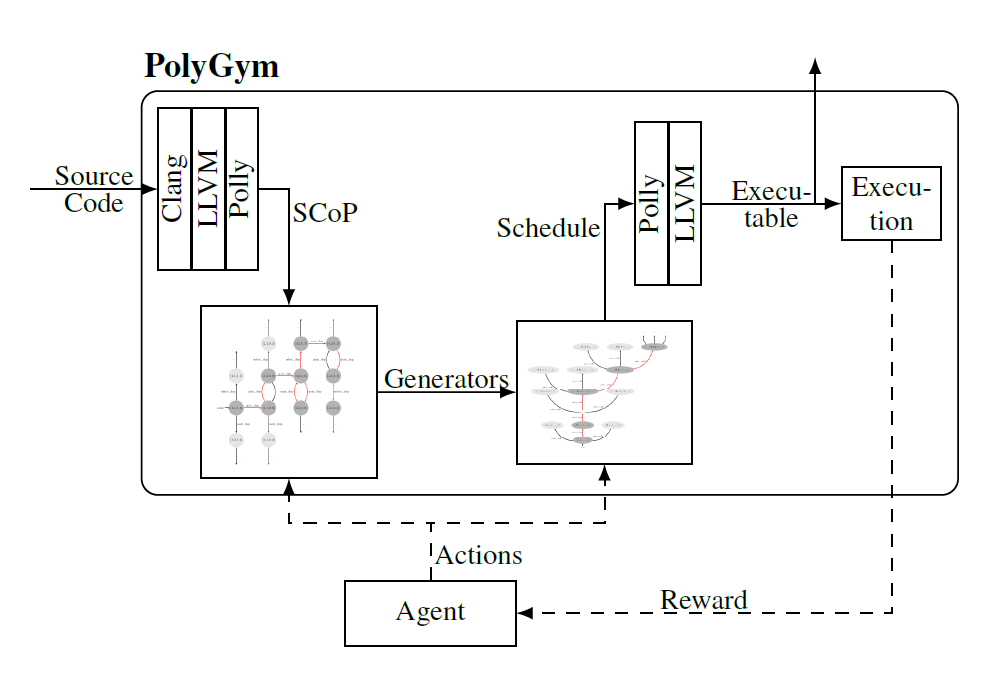
\includegraphics[width=\textwidth]{Images/PolyGym.png}
  \label{fig:polygym}  
  \caption{Polygym workflow originally demonstrated in \cite{P1}}
\end{figure}

\section{Literature Review}

Previous surveys have explored the relationship between Machine Learning and Compiler Optimizations \cite{8357388}\cite{9232934}. Several studies have also begun to examine how RL can be applied to the field of compiler optimizations. In 2014, Emani \textit{et al.} demonstrated a new approach for dynamically mapping parallel programs to varying system resources \cite{10.1007}. They used Markov Decision Process for online thread scheduling and an offline model trained based on the system environment and the structure of the code. Similar to PolyGym, CompilerGym extends the Gym interface to provide a reinforcement learning environment to researchers for compiler optimizations \cite{CompilerGym}. A recent study by Mammadli \textit{et al.} presented an excellent example of using Deep Reinforcement Learning for finding effective sequences of phase-ordering, which is a long-standing problem for compiler generators \cite{static.neural}. However, finding profitable loop transformations is a much more fine-drawn problem than finding the optimum number of threads or distributing the work on different cores. In an investigation related to current Single Instruction, Multiple Data (SIMD) architectures, Neurovectorizer \cite{NeuroVectorizer} addresses the challenge to find a good vectorization strategy with the help of Deep Reinforcement Learning. MLGO \cite{10.48550} attempted to leverage Reinforcement Learning and Evolutionary Algorithms for making decisions about function in-lining for improving code size. However, the evaluation for the code size could be less challenging than the evaluation of the heuristics focusing on the program's execution speed due to the uncertainty involved in the time taken during each execution.

All these methods, however, did not consider polyhedral optimizations. In 1993, Feautrier presented the theoretical basis of the polyhedral formulation for single and multidimensional schedules \cite{single}\cite{multi}. After more than twenty years, Pouchet \textit{et al.} proposed an iterative optimization method for systematic exploration of the schedule search space \cite{it_Single}\cite{it_multi}. Building on top of these methods, Ganser \textit{et al.} demonstrated improvements in optimization with the use of genetic algorithms in 2017 \cite{10.1145/3109482}. One year later, they showed a reduction in benchmarking efforts by using surrogate performance models, where they trained the models based on the program transformation evaluated in the previous iterative optimizations, at the cost of 15\% degradation in speed-up \cite{10.1145/3291773}. This set of methods followed the iterative approach with benchmarking, making them time-consuming. In contrast, methods such as isl\cite{isl} and Pluto\cite{Bondhugula07pluto:a} generated the models directly to find a good compilation strategy in less time. However, this approach has certain limitations. The optimization performed is still dependent on the type of loop being analyzed, and its performance can not beat the time taking iterative methods. Hence, the proposed research with Reinforcement Learning fits very well between these two approaches.

\chapter{Methodology}

\section{Clang/LLVM/Polly}

LLVM is a set of optimiser libraries built around an intermediate representation of the code, known as LLVM-IR. Like many other analyzing and optimizing tools, it uses the Clang frontend, a \textit{C} language family compiler, as a library.
Polly applies polyhedral transformations on top of this intermediate representation. It first identifies relevant regions of the code suitable for transformations, called Static Control Parts(\textit{SCoP}). It then transforms these regions into a polyhedral representation based on integer sets and maps. On this representation, it applies optimisations, for example, related to data locality and parallelism, finally converting it back into the optimised version of the executable code. As Polly analyses the low-level IR instead of the programming language itself, it is not dependent on any language or platform.

A \textit{SCoP}, generally consisting of loops and conditions, contains part of the program for which control flow and memory access can be determined at the compile time. For a loop to be identified as \textit{SCoP}, the scalar expression for the iteration count should be able to be represented as an affine function. Similarly, the memory accesses for loading and storing should also be possible to be translated into an affine expression. Polly allows the export of this polyhedral representation into a \textit{JSON} based format called \textit{jSCoP}.
This allows us to apply external optimization, which can be imported back using the same \textit{jSCoP} format.

 Figure \ref{fig:Original_Loop} showcases an example of a \textit{C} loop doing matrix multiplication. Using \textit{clang}, we can identify the \textit{SCoP} parts of the code and convert them into LLVM representation as displayed in Figure \ref{fig:Poly_Rep}. The representation consists of statements as basic building blocks. Apart from its name, a \textit{statement} consists of \textit{Domain}, \textit{Schedule} and \textit{Access}. The \textit{domain} represents a set of different loop iterations executing the statement, as a named integer set. The \textit{schedule} is an integer map which assigns a point to each iteration in a multi-dimensional space following lexicographical order. Changing the schedule will change the order in which the kernel is executed. \textit{Access} is a pair of kind and relation. The kind can be either \textit{read}, \textit{write} or may \textit{write}. The access relation maps the domain with the memory space, which generally can be represented by an affine function. Figure \ref{fig:Dependencies} explains the dependencies information extracted from the above representation, which can exist between two statements or two iterations of the same statement. When the transformations have been applied, AST can be generated from the LLVM representation as shown in Figure \ref{fig:AST} and the program can be executed.

 \section{Q-learning}

 (improve this) The value of a state can be defined as the expectation of the maximum reward which can be gained from that state, considering all the actions that can be taken in that state. To select the optimal actions, we will need to determine the values of each action and select the one with the best possible result. In a way, the value of a state corresponds to the value of the action we can take from this state, giving us the maximum possible outcome.

 The state-action value can be represented as mentioned in Equation \ref{eq:SAQV} (change this),

\begin{equation}
Q(s,a) = r(s,a) + {\gamma} max_{a'\in A} Q(s',a')
\label{eq:SAQV}
\end{equation}
 
 A Q-Network can be trained by minimising the loss function at each iteration as shown in Equation \ref{eq:DQN} (change this),

\begin{equation} L_{i}(\theta _{i}) = E_{s,a\sim\rho(\cdot)}[(y_{i} - Q(s,a;\theta _{i}))^2]
\label{eq:DQN}
\end{equation}

where \(y_{i} = E_{s'\sim\epsilon}[r+\gamma\max\limits_{{a'}}Q(s', a'; \theta_{i-1})|s, a]]\) is the target for iteration i. \(\rho(s,a)\) is the probablity distribution over states s and actions a. \(\gamma\) is the discount factor, r is the reward, and \(Q(s,a;\theta)\) is the function approximator to estimate the action-value function \cite{DBLP:journals/corr/MnihKSGAWR13}.

\section{Linear Function Approximation}

Any form of tabular learning like Q-Learning requires that we visit each and every state multiple times and apply all the available actions to estimate the correct Q-Values. However, this is not a practical approach in most real-world scenarios, especially those involving a vast state space. Also, it takes up a lot of memory to save and update the Q-table containing a large number of states and actions. One workaround to this is to approximate the Q-Functions using machine learning based on the visited states. This will allow us to approximate Q-Value for a state-action pair \textit{(s,a)} even if action \textit{a} was never applied in the state \textit{s}. It will also help us to avoid maintaining a large Q table. Linear Function Approximation \cite{P2} is a good alternative to Deep Q-Learning here, as it is not as data-hungry as Deep Leaning and requires comparatively less computation.

\begin{equation}
Q(s,a) = f_1(s) * w_1^a + f_2(s) * w_2^a + ... + f_n(s) * w_n^a 
\label{eq:Q_Approx}
\end{equation}

\begin{equation}
w_i^a = w_i^a  + {\alpha} * {\delta} * f_i(S),
\label{eq:W_Approx}
\end{equation}

\begin{equation}
{\delta} = r + {\gamma} * max_{a'} Q(s',a') - Q(s,a)
\label{eq:delta}
\end{equation}

\section{Deep Q-Learning}

\section{Agent Representation}

For the problems such as this, it is essential that the representation of the state is such that the agent is able to learn. We define two different agents here, one for the construction phase and one for the exploration. This is because the learning of the agent and the representation is completely different in both phases.

\subsection{Construction Phase}
For the construction phase, the action space consists of three actions as defined in Equation \ref{eq:CONST_ACT},
\begin{equation}
A_{con} = \{next\_dimension, \hspace{1} select\_dependency, \hspace{1} next\_dependency\}
\label{eq:CONST_ACT}
\end{equation}

(add more explanation for actions)

The states during this phase represents information of dependecies with respect to the current dimension and it can be described as Equation \ref{eq:CONST_SPC}

\begin{equation}
S_{con} = (i_{dim} ;\hspace{2} i_{dep};\hspace{2} n_d;\hspace{2} n_a)
\label{eq:CONST_SPC}
\end{equation}

In this representation, \textit{i\textsubscript{dim}} represents the current dimension, and \textit{i\textsubscript{dep}} represents the current dependency pointer. \textit{n\textsubscript{d}} stores the number of strong dependencies added in current dimensions, and \textit{n\textsubscript{a}}
represents the number of total available dependencies across all dimensions which are yet to be added strongly.

\begin{figure}[htbp]
  \centering
  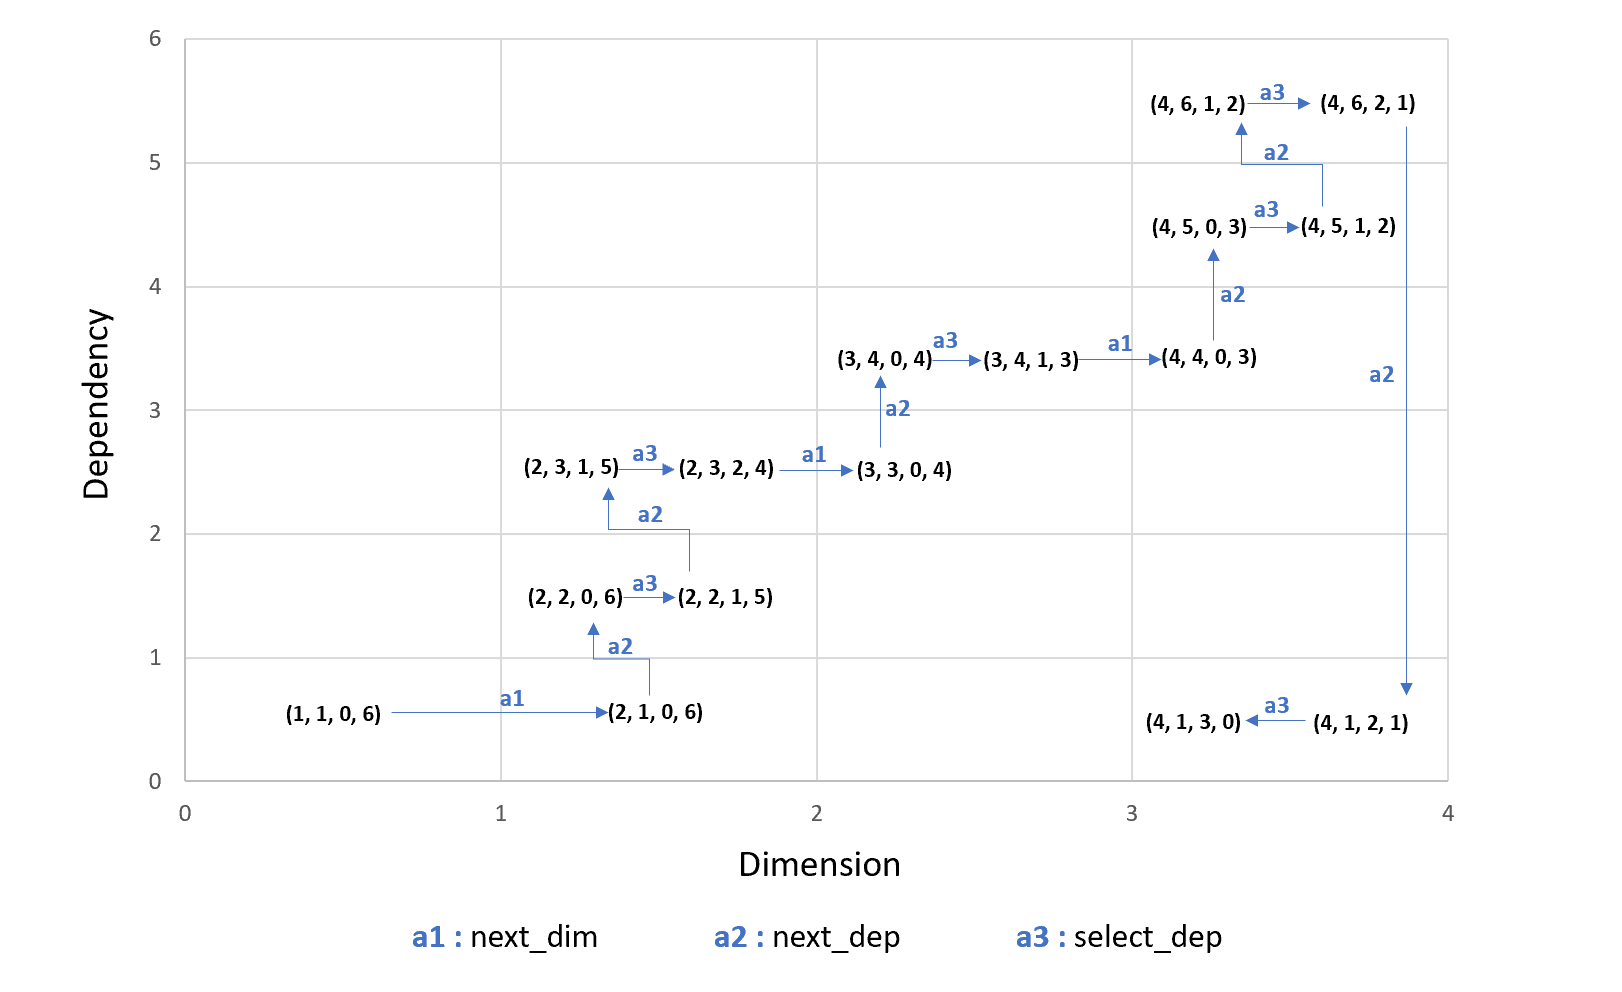
\includegraphics[width=\textwidth]{Images/Construction.png}
  \label{fig:construction}  
  \caption{Construction Phase State Representation as \textit{(i_{dim};\hspace{2}i_{dep};\hspace{2}n_d;\hspace{2}n_a)}.}
\end{figure}

Using this representation, the agent could learn if it trained and tested on the same kernel. Just within 20 iterations, we achieved an impressive speedup,  even better than the best speedup achieved during the training. While this shows that the agent's implementation is correct, more was needed to solve the problem of generalization. While testing this agent on another kernel, the performance was significantly poor.

A critical piece of information we missed was the actual parameters associated with the dependency. A dependency statement can be defined as shown below.
\begin{equation}
\begin{multlined}
[n_i, \hspace{2} n_j, \hspace{2} n_k] \hspace{2} -> \hspace{2} Stmt\_for\_body8[i_0, \hspace{2} i_1] -> Stmt\_for\_body16[i_0', \hspace{2} i_1', \hspace{2} i_2] : \\
i_0' = i_0 \hspace{2} and \hspace{2} i_1' = 0 \hspace{2} and \hspace{2} i_2 = i_1 \hspace{2} and \hspace{2} n_k > 0 \hspace{2} and \hspace{2} 0 <= i_0 < n_i \hspace{2} and \hspace{2} 2i_1<=i_0
\label{eq:DEP_STMT}
\end{multlined}
\end{equation}

The dependency defined in \ref{eq:DEP_STMT} consists of \textit{domain} variables, \textit{statements} and variable bounds which can be presented as affine functions. To provide all the inequalities a regular structure, we converted all the expressions in the format of less than equal to zero. 
For example, \textit{$0 \leq \hspace{2}$i\textsubscript{0} $< \hspace{2}$n\textsubscript{i}}  can be transformed to two different affine functions \textit{$-i\textsubscript{0} \leq \hspace{2}$0} and \textit{$i\textsubscript{0} - \hspace{2}n\textsubscript{i} + 1 \leq \hspace{2}$0}. We are allowing dependencies having four variables and four domain parameters. 
Hence we can have four variables \textit{$i_0, \hspace{2} i_1, \hspace{2} i_2, \hspace{2} i_3$}, four prime variables for the second statement \textit{$i_0', \hspace{2} i_1', \hspace{2} i_2', \hspace{2} i_3'$}, four domains \textit{$n_i, \hspace{2} n_j, \hspace{2} n_k, \hspace{2} n_m$} and one constant. Thus, inequality can be expressed in terms of the vector as shown below.\break
\begin{center}
\textit{$i\textsubscript{0} - \hspace{2}n\textsubscript{i} + 1 \leq \hspace{2}$0} \hspace{4} \verb|->| \hspace{4} [1 0 0 0 0 0 0 0 -1 0 0 0 1]
\end{center}

If we allow such 8 inequalities in one dependency statement, the number of variables used to represent the statement will be 13 * 2 * 8 = 208.

The last two parameters of the state representation, the number of strong dependencies added in the current dimension and the number of available dependencies to be added, also presented a few challenges. Firstly, they do not contain the information on which dependency was added strongly and which dependency is yet to be added. Secondly, the number of dependencies could be as high as more than 80 in the kernels such as \textit{ludcmp}. Hence, we decided to use one-hot encoding to state the added and available dependencies. For instance, if the maximum number of dependencies considered is 10, the dependencies added in the current dimension can be defined as:

\begin{center}
[1 0 0 0 1 1 0 0 0 0],
\end{center}

showcasing that dependency numbers 1, 5, and 6 are added strongly in the current dimension. Similarly, to define available dependencies, we use vector
\begin{center}
[0 1 0 0 0 0 0 0 1 1],
\end{center}

which states that dependencies 2, 9, and 10 are still not added strongly in any dimension and are still available to be added. We have considered the kernels having a maximum number of dependencies as 41 and hence, this adds 82 more variables in our state representation, taking the total variable count, including the current dimension, to 1 + 208 + 82 = 291. We have mixed and matched these representation variables, implementing dropouts, for example, using the number of available dependencies instead of one-hot encoding,  to find out which representation gives us the best result. A typical full representation of the state would look as shown below.

Comment - add actual array \break
\textit{array([ 0.,  0.,  0.,  0.,  0.,  0.,  0.,  0.,  0.,  0., -1.,  0.,  0.,
        1.,  0.,  0.,  0.,  0.,  0.,  0.,  1.,  0.,  0., -1.,  0.,  0.,
        0.,  0.,  0.,  0.,  0.,  0.,  0.,  0.,  1.,  0.,  0.,  0.,  0.,
        0.,  0.,  0.,  0.,  0., -1.,  0.,  0.,  0.,  0., -1.,  0., -1.,
        1.,  0.,  0.,  0.,  0.,  0.,  0.,  0.,  0.,  1., -1.,  0.,  0.,
        0.,  0.,  0.,  0.,  0.,  0.,  0.,  0.,  0.,  0.,  0.,  0.,  0.,
       -1.,  1., -1.,  0.,  0.,  0.,  0.,  0.,  0.,  0.,  0., -1.,  1.,
        0.,  0.,  0.,  0.,  0., -1.,  0.,  0.,  1., -1.,  2.,  0.,  0.,
        0.,  0.,  0.,  0.,  0.,  0.,  0.,  0.,  0.,  0.,  0.,  0.,  0.,
        0.,  0.,  0.,  0.,  0.,  0.,  0.,  0.,  0.,  0.,  0.,  0.,  0.,
        0.,  0.,  0.,  0.,  0.,  0.,  0.,  0.,  0.,  0.,  0.,  0.,  0.,
        0.,  0.,  0.,  0.,  0.,  0.,  0.,  0.,  0.,  0.,  0.,  0.,  0.,
        0.,  0.,  0.,  0.])}

%\textit{0 \leq i\textsubscript{0} < n\textsubscript{i}}
%\textit{-i\textsubscript{0} \leq 0}
%\textit{i\textsubscript{0} - n\textsubscript{i} + 1 \leq 0}
\subsection{Exploration Phase}

For the exploration phase, the action space consists of three actions as defined in Equation \ref{eq:CONST_ACT},
\begin{equation}
A_{con} = \{select\_coeff0, \hspace{1} select\_coeff1, \hspace{1} select\_coeff2\}
\label{eq:EXP_ACT}
\end{equation}

(add more explanation for actions)

The states during this phase represent information of dependencies with respect to the current dimension, and it can be described as Equation \ref{eq:CONST_SPC}

\begin{equation}
S_{con} = (i_{dim} ;\hspace{2} i_{dep};\hspace{2} n_d;\hspace{2} n_a)
\label{eq:CONST_SPC}
\end{equation}

\begin{figure}[htbp]
  \centering
  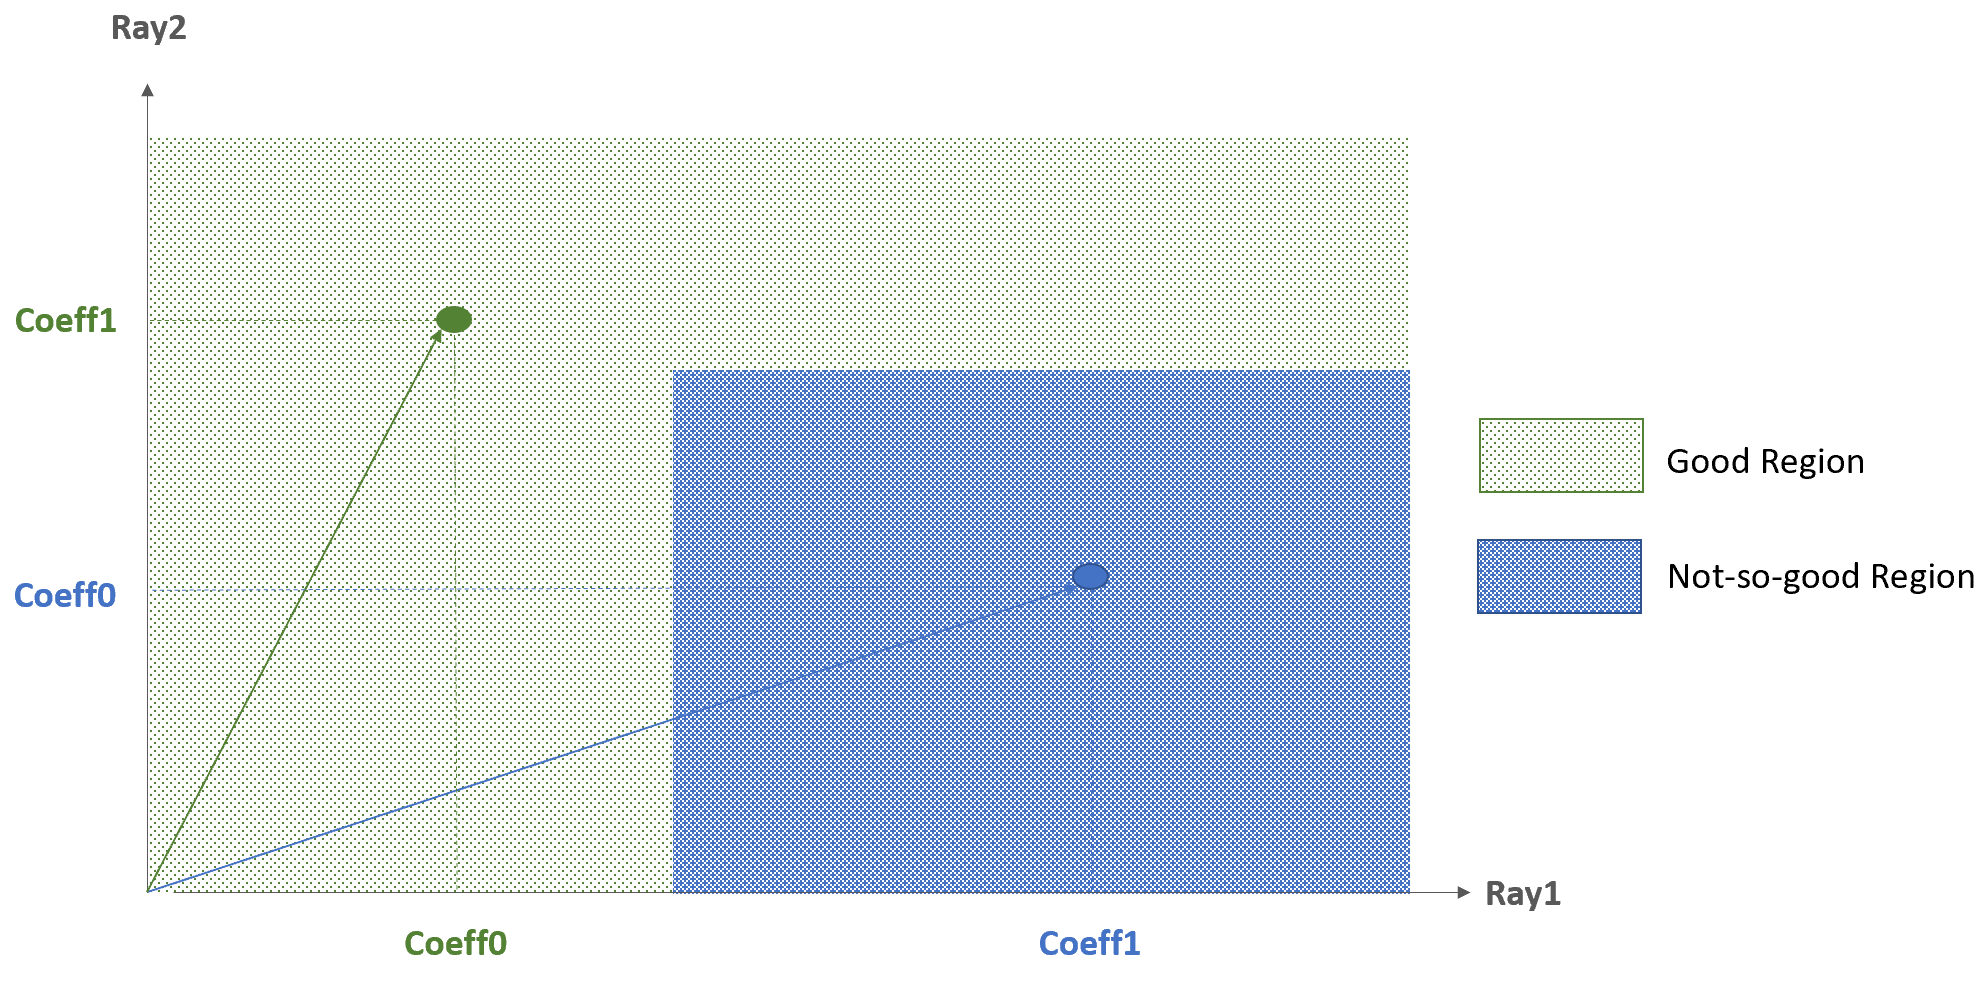
\includegraphics[width=\textwidth]{Images/Exploration.png}
  \label{fig:exploration}  
  \caption{Exploration Phase limited to one dimension and two rays for understanding}
\end{figure}

\begin{figure}[!tb]
  \centering
  \subfloat[Original Loop in C.]{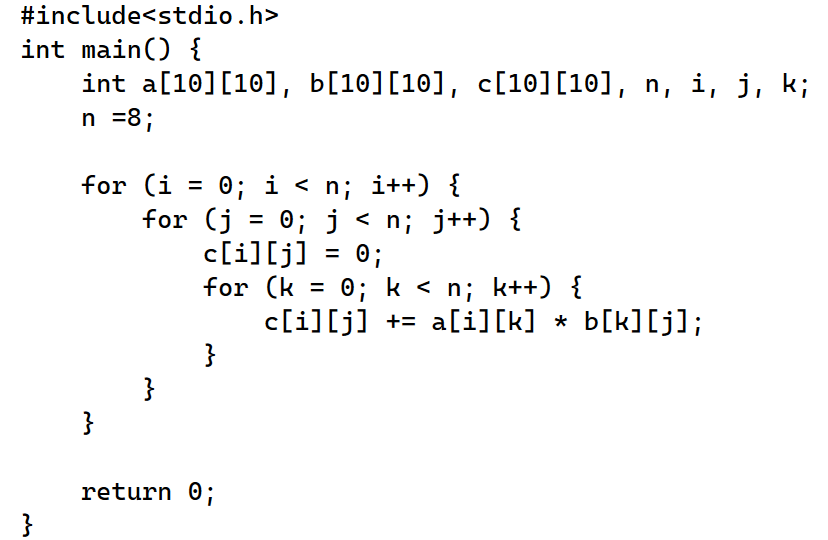
\includegraphics[width=0.5\textwidth]{Original_Loop.png}\label{fig:Original_Loop}}
  \hfill
  \subfloat[Polyhedral Representation of the identified SCoP.]{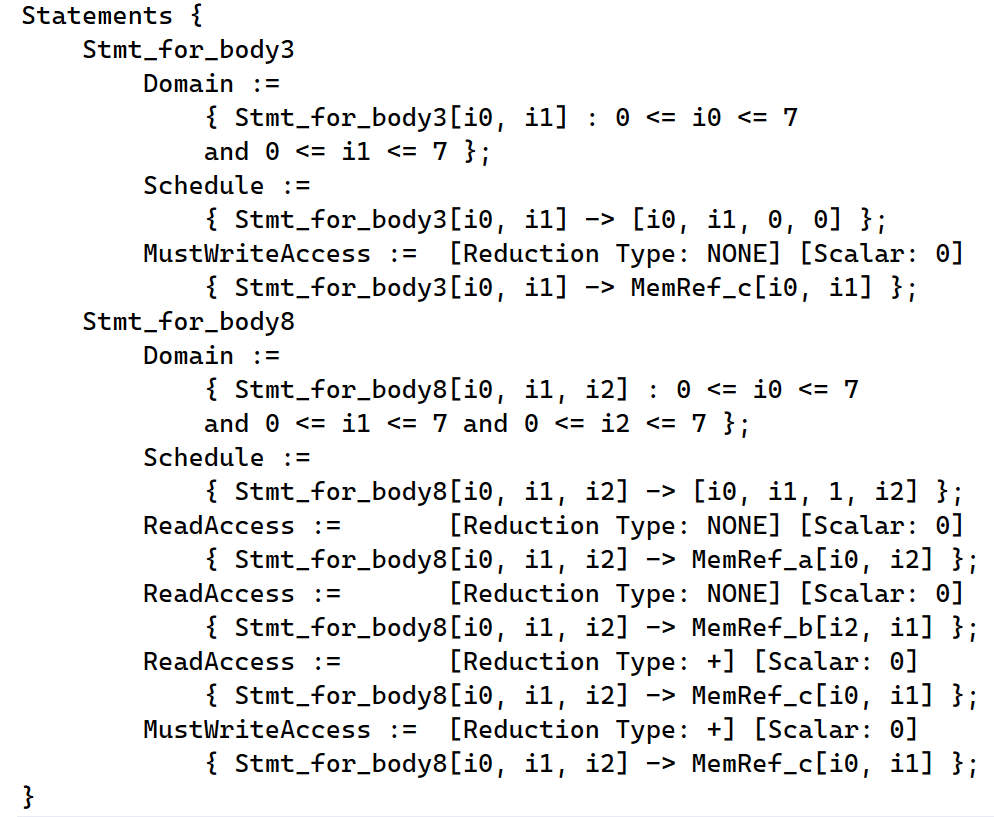
\includegraphics[width=0.5\textwidth]{Poly_Rep.png}\label{fig:Poly_Rep}}

  \centering
  \subfloat[Dependency Analysis.]{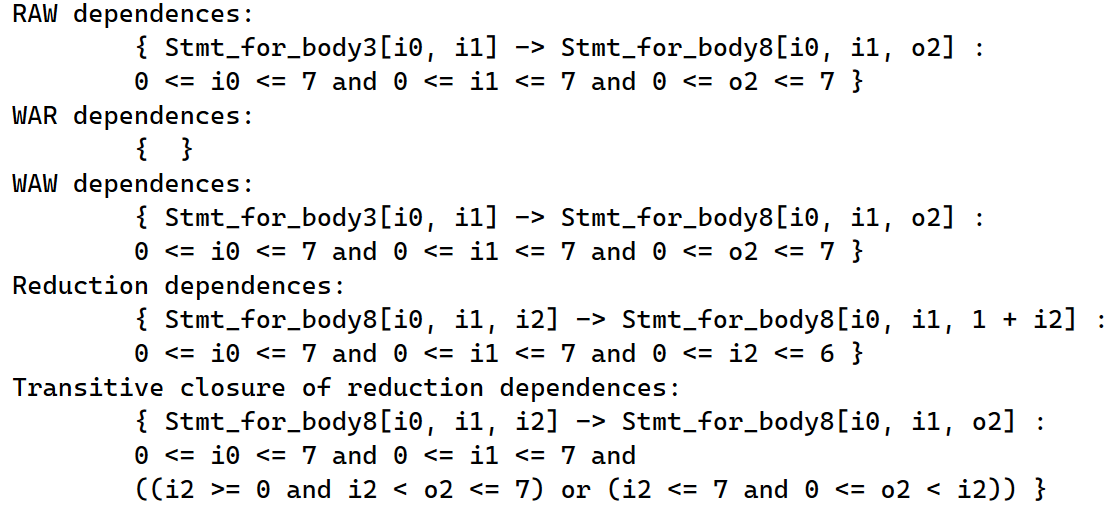
\includegraphics[width=0.5\textwidth]{Dependencies.png}\label{fig:Dependencies}}
  \hfill
  \subfloat[AST Generation from IR.]{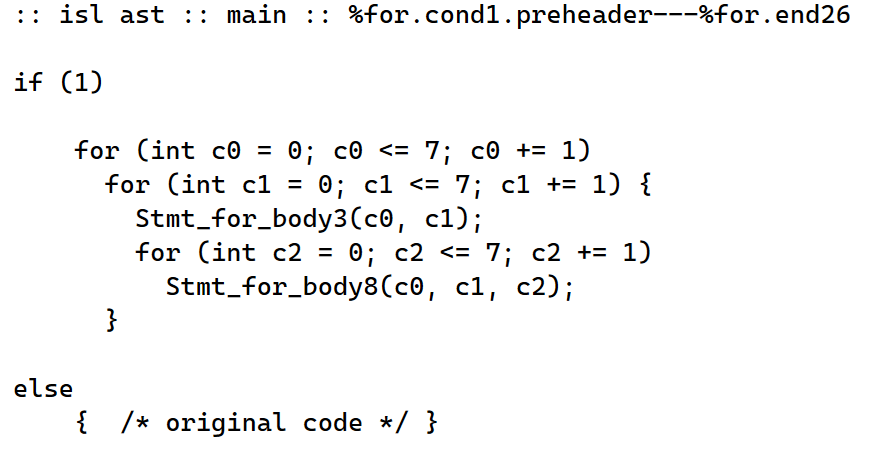
\includegraphics[width=0.5\textwidth]{AST.png}\label{fig:AST}}
  
  \caption{Generation of SCoP and AST using LLVM Polly}
\end{figure}


\chapter{Evaluation}

\section{Evaluation Setup}

\begin{figure}[htbp]
  \centering
  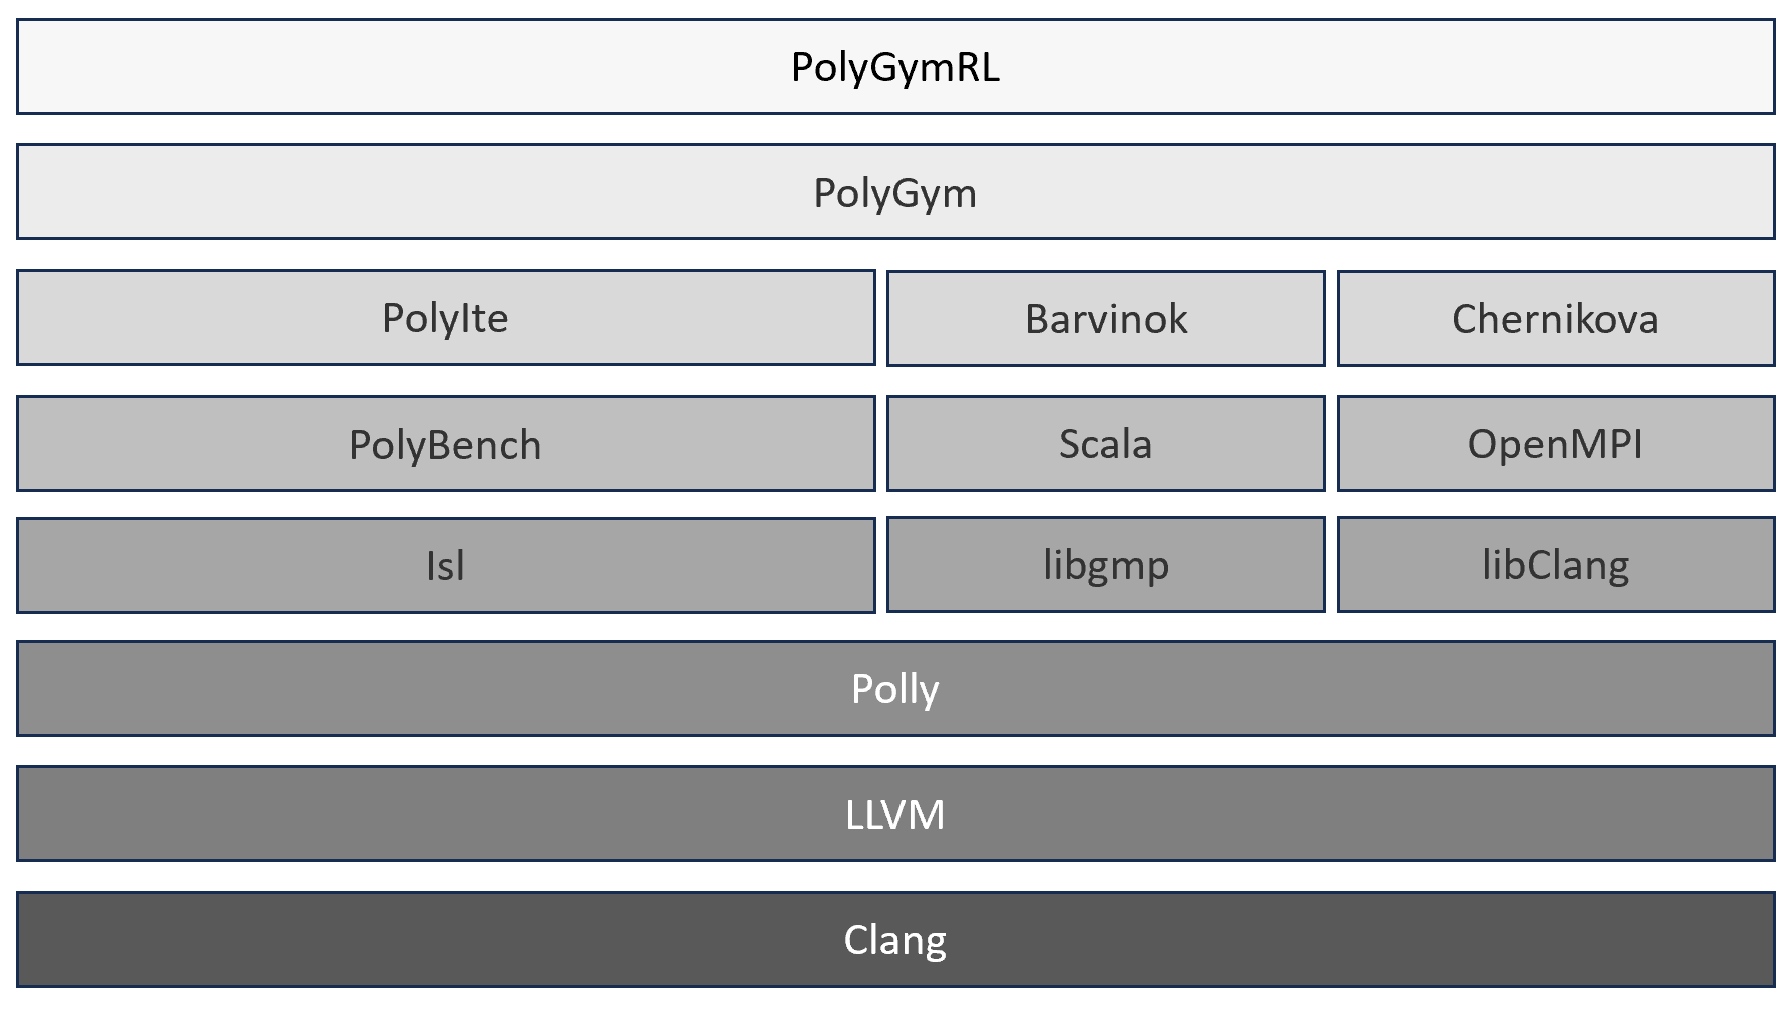
\includegraphics[width=\textwidth]{Images/PolyGymRlStack.png}
  \label{fig:stack}  
  \caption{PolyGymRL Stack}
\end{figure}

\section{Epsilon-Greedy Approach}

During the training, the agent has two choices. Either keep choosing the new actions, which is called Exploration or choose the actions giving the most reward, termed Exploitation. Exploration is good for the long run as the agent gains some new knowledge. While exploitation helps gain immediate reward, even though it might be sub-optimal. The agent can follow only one approach at a time, presenting an exploration-exploitation trade-off. In the implementation, a parameter \textit{epsilon} was kept to introduce the randomness in the training. We choose a random number from 0 to 1, if the number is less than \textit{epsilon}, then the agent explores, or else it exploits, Figure \ref{fig:randomness}.

\begin{figure}[htbp]
  \centering
  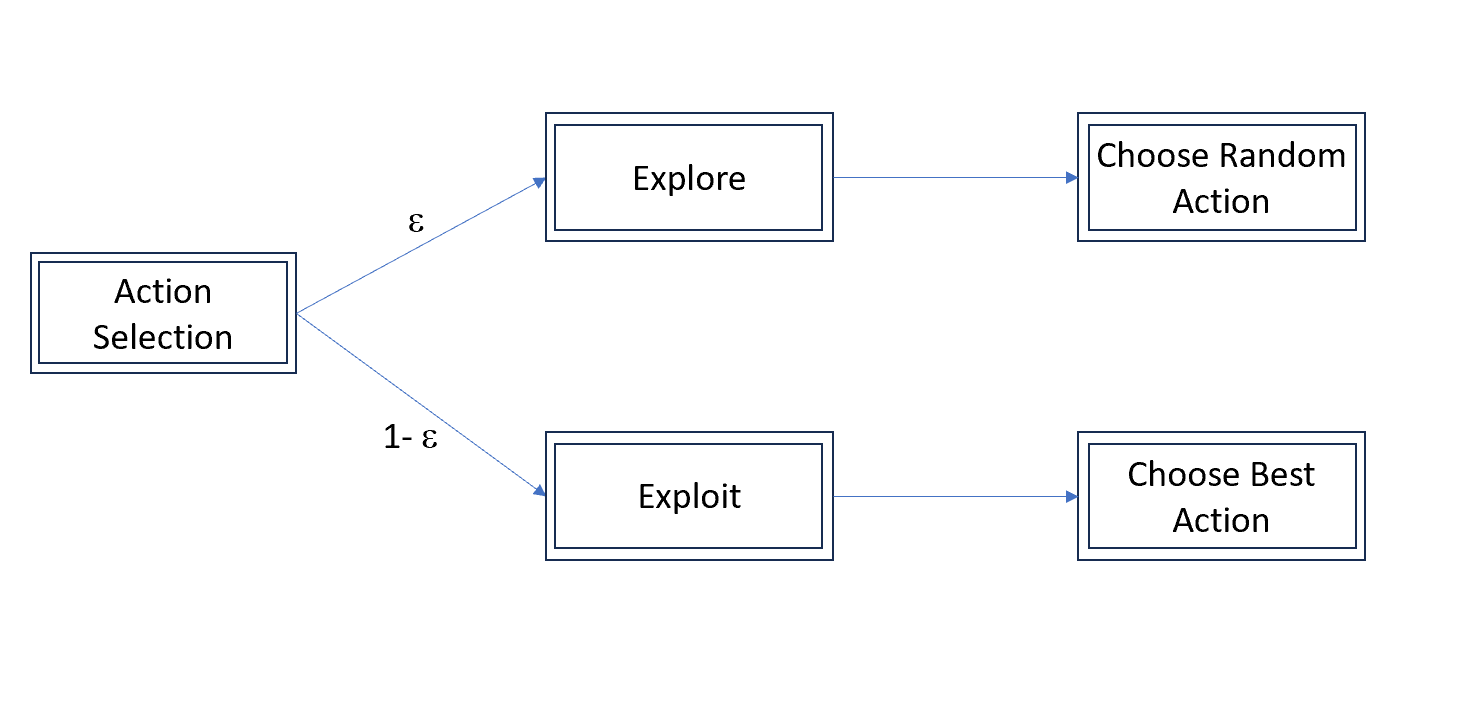
\includegraphics[width=\textwidth]{Images/Randomness.png}
  \label{fig:randomness}  
  \caption{Exploration vs Exploitation}
\end{figure}

Initially, the agent has little information, which will be a good approach to exploring more. Hence, the value of \textit{epsilon} should be higher. As the training progresses, this value should be reduced so that the agent does not spend time on actions which will not give us good rewards. However, the value should be decreased periodically. Otherwise, more exploitation in the initial phase can cause the agent to get stuck in sub-optimal space. We are reducing the \textit{epsilon} value based on the iteration of the training as described in Equation \ref{eq:RANDOMNESS}. Notably, if {$\epsilon$} value is zero, the agent always exploits the knowledge it has. On the other side, if the {$\epsilon$} value is one, the agent will always choose random actions.

((add pseudo code for epsilon implementation?))

\begin{equation}
\epsilon = 1.0 - (min{\hspace{2}}(1.0,{\hspace{2}} t / (0.9 * T))) * {\hspace{2}}0.95
\label{eq:RANDOMNESS}
\end{equation},

where t is the current iteration, and T is the total number of iterations for the training.

\section{Experience Replay Buffer}
Instead of learning as soon as we take a step in the environment, storing these transitions in a memory buffer and using them later on for learning will be useful. This is known as learning based on Experience Replay in Reinforcement learning. This approach has many advantages. Firstly, we need a good way to distribute the reward to all the state-actions pairs visited during the scheduled construction and exploration. However, we can do this only after we know the speed-up of the new schedule generated. Hence, if we have the transition history, we update the values for those state-action pairs later on. Secondly, if we are planning to train on each kernel n times, we can pick one kernel train on that kernel for n times, and move to the next kernel. However, this approach might introduce some correlation in the learning. If we store the transition history, we can randomly select the samples to break the correlation.

The base unit of this replay buffer is a transition, which can be described as per Equation \ref{eq:TRANSITION}

\begin{equation}
T = (s,\hspace{2} a,\hspace{2} r,\hspace{2} s,\hspace{2} d),
\label{eq:TRANSITION}
\end{equation}

where \textit{T} is Transition, \textit{s} is the current state in which the action is taken, \textit{a} is the action performed, \textit{r} is the reward received while performing action \textit{a} in states \textit{s}, \textit{s'} is the next state in the transition and \textit{d} is the binary value to indicate if the transition is completed, which is if the schedule is generated.

\section{Leave-one-out Evaluation}

We have conflicting priorities while distributing training and testing sets. Our training set should be large enough for the agent to learn correctly. On the other side, our testing set should be large enough to measure our agent's performance accurately. One approach to finding a middle way is to perform cross-validation, where we train and test our algorithm on the same data multiple times. We first train the agent on the training set and measure the performance on the testing set. On the next iteration, we flip the sets to train the agent on the set which was used for testing and test it on the remaining set. In general, there are more than two partitions, each time, we take a different partition for testing. In the end, we take an average of the performance of each instance. In this case, for n number of kernel examples, we tested the agent on one loop kernel after training it on n-1 kernels. Each time leave one kernel out and train the agent on other kernels, which is similar to the Leave-One-Out evaluation method. This way, our agent is exposed to the most learning, although it has increased the overall computation significantly. This method is shown in Figure \ref{fig:leave_one_out} with the help of five different kernels, however, there were more than five kernels during actual evaluation.

\begin{figure}[htbp]
  \centering
  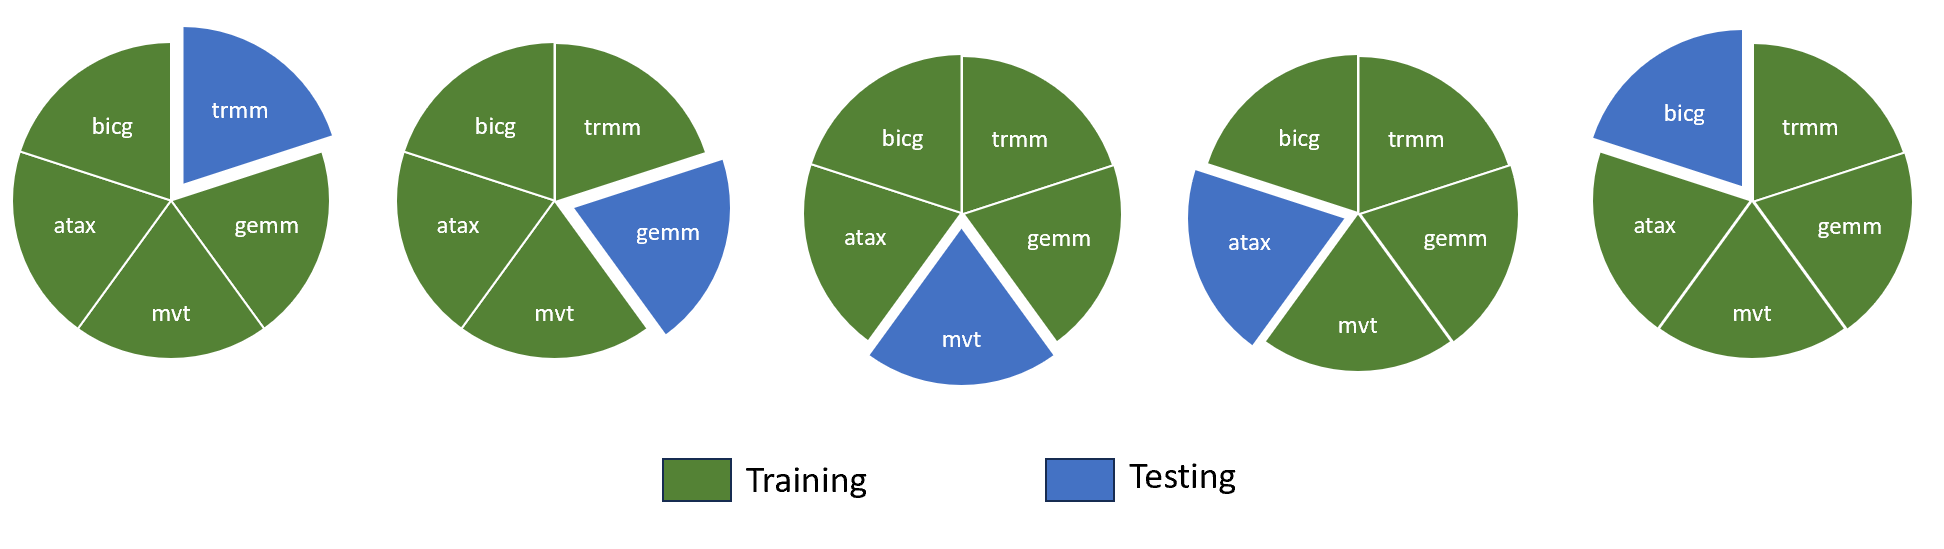
\includegraphics[width=\textwidth]{Images/Leave_One_Out.png}
  \label{fig:leave_one_out}  
  \caption{Leave-One-Out Evaluation}
\end{figure}

\chapter{Results and Discussions}
Construction time
Example of loops which performed well ---
Loops which did not perform very well , possible reasons for below average performance --- 
Chart for speedup -- 
chart for number of schedules ---
chart with hardcode xploration vs learnt exploration ---
\chapter{Conclusions}

Able to generalize the problem -- 
Using different agents for construction and exploration --
For some loops, very high performance shows the possibilities of RL for polyhedral Compilation --- 
Other advanced methods or combination of methods, trying out different state representation may help find increase in performance --- 

\section{Unresolved Issues}

More RL Methods
Combination of GA and RL
Scalability
Reward Shaping

\section{Future Work}
Deep Reinforcement learning Method
Hyperparameters search
Loop Construction Performance by performance programming an HPC
Outside Polybench Loops

\bibliographystyle{plain}
\bibliography{MLPC}


% You may delete everything from \appendix up to \end{document} if you don't need it.
\appendix

\chapter{First appendix}

\section{First section}





\end{document}
